\documentclass[tikz,border=10pt]{standalone}
\usepackage[T1]{fontenc}
\usepackage{mathpazo}
\usetikzlibrary{arrows.meta, positioning, calc, decorations.markings, bending}

\definecolor{stblue}{HTML}{7B97AD}
\definecolor{rwgold}{HTML}{B8995E}
\definecolor{sage}{HTML}{7A9A7E}
\definecolor{dkbrown}{HTML}{3D3530}
\definecolor{wmgray}{HTML}{7B7067}
\definecolor{cream}{HTML}{F9F6F0}
\definecolor{border}{HTML}{D4C9B8}

\begin{document}
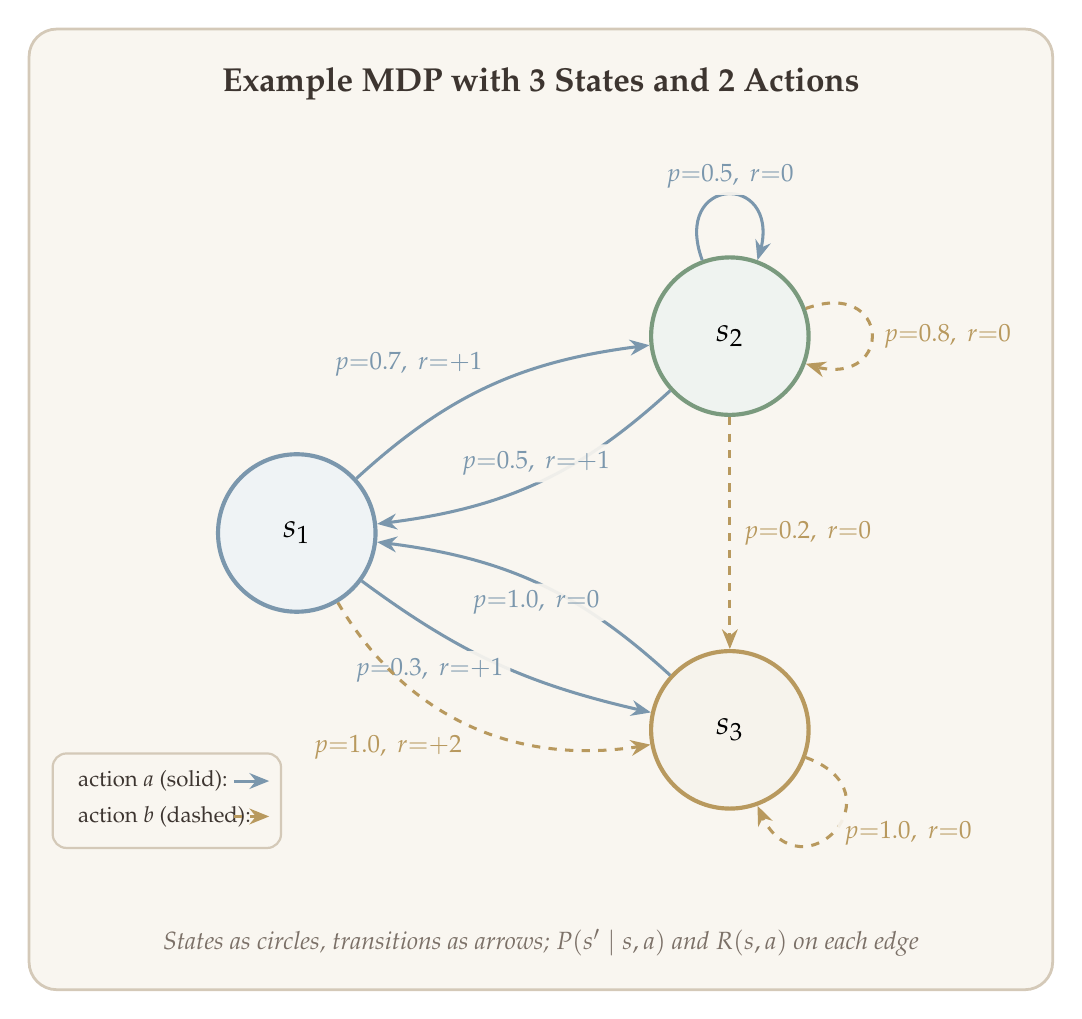
\begin{tikzpicture}[
  state/.style={circle, draw=#1, line width=1.5pt, fill=#1!12,
    minimum size=20mm, font=\large\bfseries, inner sep=0pt},
  state/.default=stblue,
  >={Stealth[length=2.5mm, width=2mm]},
  action a/.style={draw=stblue, line width=1.1pt, ->},
  action b/.style={draw=rwgold, line width=1.1pt, ->, dashed},
  elabel/.style={font=\small, fill=cream, fill opacity=0.92, text opacity=1,
    inner sep=2.5pt, rounded corners=2pt},
]

% Background — generous bounds to contain all self-loops
\fill[cream, rounded corners=10pt] (-3.4,-5.8) rectangle (9.6,6.4);
\draw[border, rounded corners=10pt, line width=1pt] (-3.4,-5.8) rectangle (9.6,6.4);

% Title
\node[font=\large\bfseries, text=dkbrown] at (3.1,5.7) {Example MDP with 3 States and 2 Actions};

% States — spread out more
\node[state=stblue] (s1) at (0,0) {$s_1$};
\node[state=sage] (s2) at (5.5,2.5) {$s_2$};
\node[state=rwgold] (s3) at (5.5,-2.5) {$s_3$};

% Legend — right side, more space
\draw[rounded corners=5pt, border, fill=cream, line width=0.8pt]
  (-3.1,-4.0) rectangle (-0.2,-2.8);
\node[font=\footnotesize, text=dkbrown, anchor=west] at (-2.9,-3.15)
  {action $a$ (solid):};
\draw[stblue, line width=1.1pt, ->] (-0.8,-3.15) -- (-0.35,-3.15);
\node[font=\footnotesize, text=dkbrown, anchor=west] at (-2.9,-3.6)
  {action $b$ (dashed):};
\draw[rwgold, line width=1.1pt, ->, dashed] (-0.8,-3.6) -- (-0.35,-3.6);

% ============================================================
% Transitions from s1
% ============================================================

% s1 -> s2 via action a (p=0.7, r=+1)
\draw[action a, bend left=18] (s1) to
  node[elabel, above left, text=stblue] {$p{=}0.7,\; r{=}{+}1$} (s2);

% s1 -> s3 via action a (p=0.3, r=+1)
\draw[action a, bend right=12] (s1) to
  node[elabel, left, text=stblue, pos=0.55] {$p{=}0.3,\; r{=}{+}1$} (s3);

% s1 -> s3 via action b (p=1.0, r=+2)
\draw[action b, bend right=35] (s1) to
  node[elabel, below left, text=rwgold] {$p{=}1.0,\; r{=}{+}2$} (s3);

% ============================================================
% Transitions from s2
% ============================================================

% s2 -> s1 via action a (p=0.5, r=+1)
\draw[action a, bend left=18] (s2) to
  node[elabel, above, text=stblue, pos=0.5] {$p{=}0.5,\; r{=}{+}1$} (s1);

% s2 -> s2 self-loop via action a (p=0.5, r=0) — loop to upper-right, inside box
\draw[action a] (s2) to[loop above, looseness=4, out=110, in=70, min distance=12mm]
  node[elabel, above=-1pt, text=stblue] {$p{=}0.5,\; r{=}0$} (s2);

% s2 -> s2 via action b (p=0.8, r=0) — loop to right
\draw[action b] (s2) to[loop right, looseness=4, out=20, in=-20, min distance=12mm]
  node[elabel, right=1pt, text=rwgold] {$p{=}0.8,\; r{=}0$} (s2);

% s2 -> s3 via action b (p=0.2, r=0)
\draw[action b] (s2) to
  node[elabel, right=2pt, text=rwgold] {$p{=}0.2,\; r{=}0$} (s3);

% ============================================================
% Transitions from s3
% ============================================================

% s3 -> s1 via action a (p=1.0, r=0)
\draw[action a, bend right=18] (s3) to
  node[elabel, below, text=stblue, pos=0.5] {$p{=}1.0,\; r{=}0$} (s1);

% s3 -> s3 self-loop via action b (p=1.0, r=0) — loop to lower-right
\draw[action b] (s3) to[loop right, looseness=4, out=-20, in=-70, min distance=12mm]
  node[elabel, right=1pt, text=rwgold] {$p{=}1.0,\; r{=}0$} (s3);

% Bottom annotation
\node[font=\small\itshape, text=wmgray] at (3.1,-5.2)
  {States as circles, transitions as arrows; $P(s' \mid s, a)$ and $R(s,a)$ on each edge};

\end{tikzpicture}
\end{document}
